\documentclass[conference]{IEEEtran}
\IEEEoverridecommandlockouts

\usepackage{cite}
\usepackage{amsmath,amssymb,amsfonts}
\usepackage{algorithm}
\usepackage{algpseudocode}
\usepackage{graphicx}
\usepackage{textcomp}
\usepackage{xcolor}
\usepackage{booktabs}
\usepackage{multirow}
\usepackage{array}
\usepackage{listings}
\usepackage{tikz}
\usetikzlibrary{arrows.meta,positioning,shapes.geometric}
\usepackage{url}
\usepackage[hidelinks]{hyperref}

\lstset{
  basicstyle=\ttfamily\scriptsize,
  breaklines=true,
  frame=single,
  numbers=left,
  numberstyle=\tiny\color{gray},
  keywordstyle=\bfseries,
  showstringspaces=false,
  xleftmargin=1.5em,
  framexleftmargin=1.2em
}

\tikzset{
  box/.style={
    draw=black!80,
    rounded corners=2pt,
    align=center,
    font=\scriptsize,
    fill=gray!6,
    inner sep=3.5pt,
    line width=0.55pt
  },
  db/.style={
    cylinder,
    cylinder uses custom fill,
    cylinder body fill=gray!6,
    cylinder end fill=gray!12,
    shape border rotate=90,
    aspect=0.22,
    draw=black!80,
    align=center,
    font=\scriptsize,
    inner sep=3pt,
    line width=0.55pt
  },
  arr/.style={
    -{Stealth[length=4.5pt,width=3.5pt]},
    line width=0.6pt,
    draw=black!80
  }
}

\begin{document}

\title{ResearcherGPT: A Multi-Agent Cognitive Framework for Hybrid Scientific Retrieval, Deterministic Grounding, Layout-Aware Extraction, and Multi-Scale Attribution}

\author{
  \IEEEauthorblockN{Archit Gupta}
  \IEEEauthorblockA{\textit{Department of Artificial Intelligence}\\
  \textit{and Data Science}\\
  Email: architag1503@gmail.com}
  \and
  \IEEEauthorblockN{Tanishq Sharma}
  \IEEEauthorblockA{\textit{Department of Artificial Intelligence}\\
  \textit{and Data Science}\\
  Email: tanishq2228@gmail.com}
}

\maketitle

\begin{abstract}
Modern scientific inquiry is constrained by rapid expansion of academic literature, rendering exhaustive synthesis, quantitative contradiction discovery, citation verification, and layout-preserving manuscript preparation difficult to automate reliably. Existing Retrieval-Augmented Generation (RAG) workflows suffer from multi-hop candidate starvation in fused rankers, unverified claim attribution under fallback paths, structural loss of vector-ruled tables during PDF parsing, and disconnected detectors inside academic integrity engines. This paper presents the hardened, evidence-verified architecture and reproducible evaluation of \emph{ResearcherGPT}, a decoupled three-tier framework spanning a Next.js/React frontend, a TypeScript/Express gateway with BullMQ and MongoDB persistence, and a Python FastAPI cognitive service executing LangGraph workflows over vector and graph storage. We implement and validate four architectural advances grounded directly in repository source code: (1) full-corpus BM25 indexing paired with additive knowledge-graph (KG) candidate-channel injection ($w \in \{0.75, 1.00\}$) inside Reciprocal Rank Fusion (RRF), overcoming the candidate ceiling of multiplicative-only graph boosts ($\beta = 1.30$); (2) a deterministic numeric-consistency and MiniLM semantic claim verifier wired directly into a post-draft quality-assurance gate; (3) geometry-aware vector-ruled table reconstruction via \texttt{pdfplumber} alongside canonical structural validation; and (4) unified Winnowing ($w{=}4$, five-token shingles) plus MinHash exact matching with shared structural, mathematical formula, and code extraction. Across five offline, seed-fixed evaluation suites (60 indexed documents / 180 chunks with 75 stratified queries, 90 balanced claims, 60 plagiarism pairs plus 30 AI/human samples, 15 synthetic two-column PDFs, and 5 executions of the compiled 13-node LangGraph pipeline) analyzed with 2,000-resample 95\% bootstrap confidence intervals and paired Wilcoxon tests, KG candidate-channel fusion raises overall Recall@5 from 0.687 (pre-fix baseline) to 0.760 at $w{=}0.75$ ($p{=}0.000911$) and 0.840 at $w{=}1.00$ ($p{=}0.000290$), lifting multi-hop KG Recall@5 from 0.060 to 0.520 without degrading lexical MRR (0.833) or semantic Recall@5 (1.000). Hybrid claim verification improves 3-way grounding accuracy from 0.667 to 0.944 (binary accuracy 0.989, false positive rate 0.033); Winnowing and shared structural extraction raise integrity F1 from 0.750 to 0.889 (1.000 detection on patchwriting and math/code plagiarism with zero clean-control false positives); and \texttt{pdfplumber} raises ruled-table recall from 0.000 to 1.000 (74.88~ms/PDF). We report remaining gaps transparently alongside a structured technical roadmap.
\end{abstract}

\begin{IEEEkeywords}
Multi-agent systems, retrieval-augmented generation, knowledge graphs, reciprocal rank fusion, scientific paper synthesis, MinHash, Winnowing, academic integrity.
\end{IEEEkeywords}

\section{Introduction}
The velocity of peer-reviewed publication has surpassed manual comprehension capacity. Across computational sciences, vast numbers of preprints and journal articles are indexed annually across arXiv, IEEE Xplore, ACM Digital Library, and PubMed. Scholars must aggregate dense experimental literature, isolate methodological contributions, detect empirical contradictions between baselines, identify open research gaps, and compile publication-compliant manuscripts.

Large Language Models (LLMs) demonstrate strong linguistic fluency, yet applying naive prompts or conventional Retrieval-Augmented Generation (RAG)~\cite{lewis2020rag} pipelines to scholarly synthesis exposes four critical system limitations verified across real software deployments:
\begin{itemize}
  \item \emph{Context fragmentation and multi-hop candidate starvation:} Standard dense vector retrieval partitions manuscripts into token chunks, severing cross-paper ontological relations such as a method evaluated on a benchmark dataset and compared against prior baselines. Even when hybrid retrievers combine dense search with Okapi BM25~\cite{robertson2009bm25} and graph boosting via Reciprocal Rank Fusion (RRF)~\cite{cormack2009rrf}, implementation defects---such as scoring BM25 solely across top-$2k$ dense results or applying graph multipliers solely to pre-existing union candidates---prevent unseen exact-match and multi-hop documents from entering top-$K$ rankings.
  \item \emph{Bibliographic and quantitative hallucination:} Generative models may emit mismatched numerical metrics, invert improvement directions, or attribute assertions to citations that fail to substantiate them~\cite{min2023factscore}. Worse, fallback verification logic that blindly marks any claim \texttt{verified} whenever evidence chunks are non-empty creates complete false-positive blindness.
  \item \emph{Loss of scientific tables and layout structures:} Plain-text PDF parsing flattens multi-column reading order and strips vector-ruled numerical tables, discarding structured headers and cell matrices required for empirical comparison.
  \item \emph{Fragmented academic integrity detectors:} Global Jaccard estimation via MinHash~\cite{broder1997minhash} dilutes short localized patchwrites inside multi-page papers unless paired with positional Winnowing~\cite{schleimer2003winnowing}, while non-prose comparison modules checking headings, equations, and code blocks fail silently if local reference extraction omits structural fields.
\end{itemize}

We present the hardened, evidence-verified realization of \emph{ResearcherGPT}, a distributed multi-agent workspace and scholarly synthesis framework engineered to eliminate these defects while maintaining strict backward compatibility and full offline reproducibility.

\subsection{Problem Statement and Scope}
An autonomous scholarly synthesis and attribution assistant must satisfy five operational criteria grounded in executable verification:
\begin{enumerate}
  \item \emph{Relational grounding:} Combine semantic vector intent, full-corpus lexical precision, and explicit knowledge-graph candidate injection so multi-hop relational evidence enters fused top-$K$ rankings reliably without harming single-hop precision.
  \item \emph{Deterministic attribution veracity:} Validate atomic empirical claims against retrieved chunks using combined semantic affinity and signed/magnitude numeric consistency checks, flagging numeric inversions and dangling citation identifiers deterministically even offline.
  \item \emph{Structural and tabular integrity:} Recover multi-column reading order, DOI identifiers, and two-dimensional vector-ruled table matrices alongside normalized section headings and deduplicated references.
  \item \emph{Fault-tolerant deterministic orchestration:} Coordinate thirteen specialized agent nodes across typed shared state with environment-guarded multi-provider routing and real post-draft quality-assurance reporting.
  \item \emph{Multi-scale academic integrity:} Unify MinHash global resemblance, Winnowing local fingerprinting, shared structural/formula/code extraction, citation network coupling, semantic cosine checks, and AI writing heuristics behind fail-closed authentication.
\end{enumerate}

To evaluate these criteria rigorously, we formulate four measurable research questions (\textbf{RQ1}--\textbf{RQ4}) and corresponding hypotheses (\textbf{H1}--\textbf{H4}):
\begin{itemize}
  \item \textbf{RQ1 (Retrieval):} Does full-corpus BM25 paired with additive KG candidate-channel injection ($w > 0$) overcome candidate-set starvation on exact-identifier and multi-hop KG queries relative to dense-only, pre-fix buggy hybrid (\texttt{CR-1}), and multiplicative-only KG baselines? \emph{(H1: KG channel weights $w \in \{0.75, 1.00\}$ significantly increase multi-hop Recall@5 and overall MRR without single-hop regression.)}
  \item \textbf{RQ2 (Claim Grounding):} Does combining \texttt{all-MiniLM-L6-v2} semantic affinity with explicit numeric tolerance and sign-inversion rules eliminate blind fallback false positives? \emph{(H2: Hybrid MiniLM+numeric verification achieves $>0.90$ three-way accuracy and $<0.05$ false-positive support rate.)}
  \item \textbf{RQ3 (Integrity Detection):} Does uniting Winnowing ($w{=}4$, five-token shingles) with MinHash and shared structural/formula/code extraction recover patchwrites and non-prose reuse at zero false-positive cost? \emph{(H3: Post-fix integrity matching achieves $1.00$ detection on patchwrite and math/code strata and $0.00$ FPR on clean controls, while isolating sparse TF-IDF limits on semantic paraphrases.)}
  \item \textbf{RQ4 (Layout Ingestion):} Does coordinate/vector-line parsing via \texttt{pdfplumber} recover quantitative tables missed by text-block extractors within sub-100~ms synthetic document latency? \emph{(H4: Ruled-table extraction lifts recall from $0.00$ to $1.00$ with $1.00$ exact cell-row parity.)}
\end{itemize}

\subsection{System Overview}
ResearcherGPT implements a decoupled three-tier architecture (Fig.~\ref{fig:arch}):
\begin{itemize}
  \item \emph{Client tier (\texttt{client/}):} Next.js and React interface with Zustand state management, a TipTap rich-text manuscript canvas, KaTeX math previewing, and a dual-schema integrity reporting UI compatible with both Express and Python payload contracts.
  \item \emph{Gateway and integrity tier (\texttt{server/}):} Node.js, TypeScript, and Express API tier integrating BullMQ and Redis job scheduling, MongoDB persistence, fail-closed production authentication guards, and the multi-scale TypeScript integrity engine.
  \item \emph{Cognitive AI tier (\texttt{ai-service/}):} Python FastAPI microservice hosting PyMuPDF and \texttt{pdfplumber} ingestion, Qdrant and in-memory cosine vector stores, Neo4j and in-memory property-graph traversal, hybrid RRF+KG search, a 13-node compiled LangGraph workflow, numeric-consistent claim verification, \texttt{PaperValidator}, and \texttt{FormaTeX} compilation.
\end{itemize}

The principal engineering and scientific contributions of this work are:
\begin{enumerate}
  \item \emph{Resolution of retrieval candidate starvation:} Diagnosing and fixing sub-corpus BM25 leakage (\texttt{CR-1}) and introducing additive KG candidate-channel RRF (Eq.~\eqref{eq:rrf_kg}), yielding statistically verified Recall@5 gains from 0.687 to 0.760 ($w{=}0.75$) and 0.840 ($w{=}1.00$).
  \item \emph{Deterministic claim grounding and QA auditing:} Replacing vacuous verification stubs with MiniLM + numeric consistency checking (\texttt{0.944} 3-way accuracy) integrated into post-draft LangGraph state emission.
  \item \emph{Unified multi-scale integrity and auth hardening:} Activating dead-code Winnowing and reference structural extraction (lifting integrity F1 from 0.750 to 0.889), enforcing fail-closed production auth, and removing hardcoded API key literals.
  \item \emph{Layout-aware table parsing and open reproducibility:} Integrating \texttt{pdfplumber} matrix extraction (\texttt{1.000} ruled-table recall), canonical LaTeX validation, and five seed-fixed evaluation suites generating CSV/JSON logs and 2,000-resample bootstrap CIs.
\end{enumerate}

\section{Literature Review and Related Work}

\subsection{Evolution of Retrieval-Augmented Generation}
Retrieval-Augmented Generation was formalized by Lewis et al.~\cite{lewis2020rag} to ground language model outputs in retrieved external documents, mitigating parametric hallucinations on knowledge-intensive queries. Subsequent neural retrieval adopted bi-encoder dense passage architectures including Dense Passage Retrieval (DPR)~\cite{karpukhin2020dpr}, Sentence-BERT~\cite{reimers2019sbert}, and compact attention-distilled encoders such as MiniLM~\cite{wang2020minilm}, indexed via Hierarchical Navigable Small World (HNSW) approximate nearest-neighbor graphs~\cite{malkov2020hnsw}. When neural embeddings are unavailable or offline, signed feature hashing~\cite{weinberger2009hashing} maps token $n$-grams into compact fixed-dimensional vectors preserving inner products in expectation.

Dense encoders capture semantic paraphrases effectively but struggle with exact alphanumeric identifiers, thresholds, and dataset codes where sparse Okapi BM25~\cite{robertson2009bm25} remains superior. Reciprocal Rank Fusion (RRF)~\cite{cormack2009rrf} aggregates heterogeneous ranked lists without brittle score calibration. Beyond flat chunk retrieval, GraphRAG~\cite{edge2024graphrag} leverages entity-relation communities for query-focused summarization, while specialized scholarly agents---including PaperQA2~\cite{skarlinski2024paperqa2} (iterative search, gather, and contextual reranking) and OpenScholar~\cite{asai2024openscholar} (large-scale open retrieval with self-feedback)---advance automated literature synthesis. Unlike PaperQA2 and OpenScholar, ResearcherGPT embeds project-scoped retrieval inside an integrated drafting and integrity platform and demonstrates why multiplicative KG boosts alone fail when multi-hop neighbors fall outside dense candidate pools.

\subsection{Multi-Agent Systems and Attribution Verification}
Multi-agent orchestration frameworks such as AutoGen~\cite{wu2023autogen}, CrewAI~\cite{moura2024crewai}, and LangGraph~\cite{langchain2024langgraph,pearson2026langgraph} decompose complex reasoning into role-specific modules communicating over typed state graphs. However, synthesized scholarly prose still risks misquoting quantitative results or citing unsupported sources unless each sentence undergoes atomic verification akin to FActScore~\cite{min2023factscore}. ResearcherGPT pairs sequential LangGraph execution with lightweight deterministic numeric-consistency and MiniLM grounding so quantitative inversions are caught cleanly even without external LLM judges.

\subsection{Layout-Aware Document Extraction}
Academic PDFs store structure implicitly via character coordinates, font spans, and vector drawing primitives. PyMuPDF~\cite{pymupdf2024docs} recovers reading-ordered text blocks and metadata quickly, while \texttt{pdfplumber}~\cite{singervine2024pdfplumber} reconstructs explicit horizontal/vertical line grids into structured table cells. Coupling both extractors with canonical structural sanitization ensures quantitative tables survive into downstream drafting.

\subsection{Plagiarism Detection and Academic Integrity}
As categorized by Folt\'{y}nek, Meuschke, and Gipp~\cite{foltynek2019plagiarism}, misconduct detection requires complementary lexical, structural, mathematical, and bibliographic signals. MinHash~\cite{broder1997minhash} estimates document-wide Jaccard overlap efficiently, whereas Winnowing~\cite{schleimer2003winnowing} guarantees contiguous substring detection using rolling window minima independent of document length. Structural and mathematical expression comparisons parallel Zhang--Shasha ordered tree-edit distance~\cite{zhang1989ted}, while metadata disambiguation draws on OpenAlex~\cite{priem2022openalex} and Crossref~\cite{hendricks2020crossref}. Table~\ref{tab:related_comparison} positions ResearcherGPT relative to closest frameworks.

\begin{table*}[t]
\centering
\caption{Critical Positioning Relative to Closest Literature Synthesis and RAG Frameworks}
\label{tab:related_comparison}
\footnotesize
\setlength{\tabcolsep}{4pt}
\begin{tabular}{p{2.3cm}p{2.7cm}p{2.6cm}p{2.6cm}p{2.5cm}p{2.4cm}}
\toprule
\textbf{System} & \textbf{Retrieval Mechanism} & \textbf{Multi-Hop Strategy} & \textbf{Claim Grounding} & \textbf{PDF \& Table Parsing} & \textbf{Integrity Engine} \\
\midrule
PaperQA2~\cite{skarlinski2024paperqa2} & Dense + BM25 + LLM reranking & Iterative agent query loops & LLM RCS evidence grading & Full-text PDF chunking & Not integrated \\
OpenScholar~\cite{asai2024openscholar} & Dense + trained OpenScholar-Reranker & Corpus-wide multi-pass RAG & Self-feedback citation critique & Pre-indexed scholarly text & Not integrated \\
GraphRAG~\cite{edge2024graphrag} & Vector + Leiden graph communities & Global map-reduce summaries & General QA (non-bibliographic) & Plain text chunks & Not integrated \\
\textbf{ResearcherGPT (Ours)} & \textbf{MiniLM + Full-Corpus BM25 + KG-Ch.\ RRF} & \textbf{KG Candidate-Channel Injection + $\beta{=}1.30$} & \textbf{MiniLM + Bigram + Numeric Consistency QA} & \textbf{PyMuPDF + \texttt{pdfplumber} 2D Matrices} & \textbf{MinHash + Winnowing + Struct/Math/Code} \\
\bottomrule
\end{tabular}
\end{table*}

\section{Proposed Methodology}
The verified ResearcherGPT methodology comprises four core mathematical components: full-corpus hybrid retrieval with KG candidate-channel injection, linear 13-node state orchestration with provider fallback, numeric-consistent hybrid claim grounding, and multi-scale integrity verification.

\begin{figure}[t]
\centering
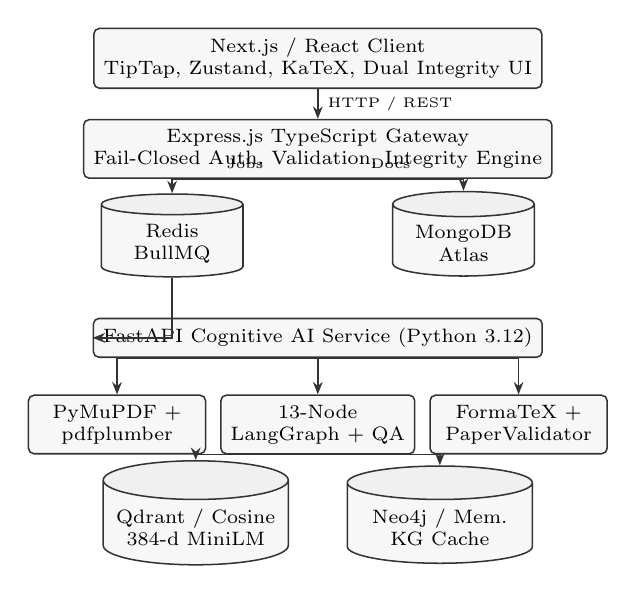
\begin{tikzpicture}
  \node[box, minimum width=5.6cm] (client) at (0, 0) {Next.js / React Client\\TipTap, Zustand, KaTeX, Dual Integrity UI};
  \node[box, minimum width=5.6cm] (gateway) at (0, -1.15) {Express.js TypeScript Gateway\\Fail-Closed Auth, Validation, Integrity Engine};
  \node[db, minimum width=1.8cm] (redis) at (-1.85, -2.35) {Redis\\BullMQ};
  \node[db, minimum width=1.8cm] (mongo) at (1.85, -2.35) {MongoDB\\Atlas};
  \node[box, minimum width=5.6cm] (fastapi) at (0, -3.55) {FastAPI Cognitive AI Service (Python 3.12)};
  \node[box, minimum width=2.25cm] (ingest) at (-2.55, -4.65) {PyMuPDF +\\pdfplumber};
  \node[box, minimum width=2.35cm] (lang) at (0, -4.65) {13-Node\\LangGraph + QA};
  \node[box, minimum width=2.25cm] (formatex) at (2.55, -4.65) {FormaTeX +\\PaperValidator};
  \node[db, minimum width=2.35cm] (qdrant) at (-1.55, -5.95) {Qdrant / Cosine\\384-d MiniLM};
  \node[db, minimum width=2.35cm] (neo4j) at (1.55, -5.95) {Neo4j / Mem.\\KG Cache};

  \draw[arr] (client) -- node[right,font=\tiny]{HTTP / REST} (gateway);
  \draw[arr] (gateway.south) -| node[pos=0.25,above,font=\tiny]{Jobs} (redis.north);
  \draw[arr] (gateway.south) -| node[pos=0.25,above,font=\tiny]{Docs} (mongo.north);
  \draw[arr] (redis.south) |- (fastapi.west);
  \draw[arr] (fastapi.south) -| (ingest.north);
  \draw[arr] (fastapi.south) -- (lang.north);
  \draw[arr] (fastapi.south) -| (formatex.north);
  \draw[arr] (lang.south) -| (qdrant.north);
  \draw[arr] (lang.south) -| (neo4j.north);
\end{tikzpicture}
\caption{Verified three-tier architecture of ResearcherGPT connecting presentation, Express integrity gateway, and FastAPI cognitive services.}
\label{fig:arch}
\end{figure}

\subsection{Full-Corpus Hybrid and KG-Channel RRF Retrieval}
Let $q$ denote a scholarly query and let
\begin{equation}
\mathcal{C}_p = \{c_1, c_2, \dots, c_N\}
\end{equation}
denote all indexed chunks extracted from papers inside workspace project $p$, with each chunk $c_i$ carrying \texttt{paper\_id}$(c_i)$, \texttt{chunk\_index}, \texttt{embedding\_model}, and \texttt{embedding\_dim}.

\subsubsection{Dense Semantic Retrieval and Feature-Hash Fallback}
By default, chunks are embedded into $d{=}384$ unit vectors via \texttt{all-MiniLM-L6-v2}. When neural weights are offline or disabled, \texttt{get\_fast\_fallback\_embedding()} applies deterministic signed feature hashing~\cite{weinberger2009hashing} over lowercased unigrams and adjacent bigrams:
\begin{equation}
v_i[h(g) \bmod d] \mathrel{+}= s(g), \qquad \hat{v}_i = \frac{v_i}{\|v_i\|_2},
\end{equation}
where $h(g)$ and $s(g) \in \{-1, +1\}$ are computed using keyed \texttt{blake2b} digests and $d{=}384$. Query cosine similarity is
\begin{equation}
S_{\text{dense}}(q, c_i) = \hat{q}^\top \hat{v}_i.
\end{equation}
Search executes via Qdrant HNSW or identical-API in-memory storage when Qdrant is unreachable, enforcing dimension parity and guarding collection schema drops behind \texttt{QDRANT\_RECREATE\_ON\_MISMATCH=true} to return top-$2K$ dense ranking $\mathcal{R}_D$.

\subsubsection{Full-Corpus Sparse Lexical Retrieval (CR-1 Fix)}
To eliminate sub-corpus starvation in the pre-fix baseline (\texttt{CR-1}), \texttt{hybrid\_retriever.py} retrieves all project chunks $\mathcal{C}_p$ via \texttt{scroll\_project\_chunks(p)}, tokenizes both document-frequency maps and queries with consistent \texttt{\_tokenize\_bm25}, computes Okapi BM25~\cite{robertson2009bm25} ($k_1{=}1.5$, $b{=}0.75$):
\begin{equation}
\text{BM25}(q, c_i) = \sum_{j=1}^{m} \text{IDF}(t_j)
\frac{f(t_j, c_i)(k_1 + 1)}{f(t_j, c_i) + k_1\!\left(1 - b + b \frac{|c_i|}{\text{avgdl}}\right)},
\end{equation}
with inverse document frequency
\begin{equation}
\text{IDF}(t_j) = \ln\!\left(\frac{N - n(t_j) + 0.5}{n(t_j) + 0.5} + 1\right),
\end{equation}
and filters strictly to $\text{BM25}(q, c_i) > 0$ to construct $\mathcal{R}_B$.

\subsubsection{Knowledge-Graph Association}
Let $G_p = (V_p, E_p)$ be the project's property graph in Neo4j or \texttt{Neo4jClient.in\_memory\_graphs}, with vertices partitioned across papers, authors, methods, datasets, metrics, technologies, and concepts:
\begin{equation}
V_p = V_{\text{paper}} \cup V_{\text{author}} \cup V_{\text{method}} \cup V_{\text{dataset}} \cup V_{\text{concept}}.
\end{equation}
Query tokens longer than three characters match non-paper entity nodes via Cypher traversal (Listing~\ref{lst:cypher}) or in-memory term lookup in \texttt{query\_papers\_by\_terms()}, yielding ranked KG paper IDs $\mathcal{K}_q \subseteq V_{\text{paper}}$ sorted by matched entity hit count.

\begin{lstlisting}[language=SQL,caption={Executed Neo4j Cypher traversal in graph\_service.py.},label={lst:cypher}]
MATCH (e:Entity {projectId: $projectId})
WHERE toLower(e.label) IN $words
  AND NOT e.type = 'paper'
MATCH (e)-[:RELATION]-
  (p:Entity {type: 'paper', projectId: $projectId})
RETURN DISTINCT p.id AS paperId
\end{lstlisting}

\subsubsection{Extended RRF with KG Candidate-Channel Injection}
Resolving the structural ceiling of purely multiplicative KG boosting ($\beta{=}1.30$ on $\mathcal{R}_D \cup \mathcal{R}_B$ alone), we score each candidate paper $d \in \mathcal{R}_D \cup \mathcal{R}_B \cup \mathcal{K}_q$ (Fig.~\ref{fig:retrieval_pipe}) via extended RRF ($k{=}60$):
\begin{equation}
\label{eq:rrf_kg}
\begin{aligned}
S_{\text{RRF+KG}}(d) ={}& \gamma(d)\!\left(\frac{\mathbb{I}[d \in \mathcal{R}_D]}{60 + r_D(d)} + \frac{\mathbb{I}[d \in \mathcal{R}_B]}{60 + r_B(d)}\right) \\
& + w \cdot \frac{\mathbb{I}[d \in \mathcal{K}_q]}{60 + r_K(d)},
\end{aligned}
\end{equation}
where $r_D(d), r_B(d), r_K(d) \ge 1$ denote 1-based paper ranks across dense, full-corpus BM25, and KG candidate lists,
\begin{equation}
\gamma(d) =
\begin{cases}
1.30, & d \in \mathcal{K}_q,\\
1.00, & \text{otherwise},
\end{cases}
\end{equation}
and $w \ge 0$ controls additive KG channel injection (deployed default $w{=}0.75$; equal weight $w{=}1.00$). When $w{=}0$, Eq.~\eqref{eq:rrf_kg} reduces exactly to multiplicative-only rescoring.

\begin{figure}[t]
\centering
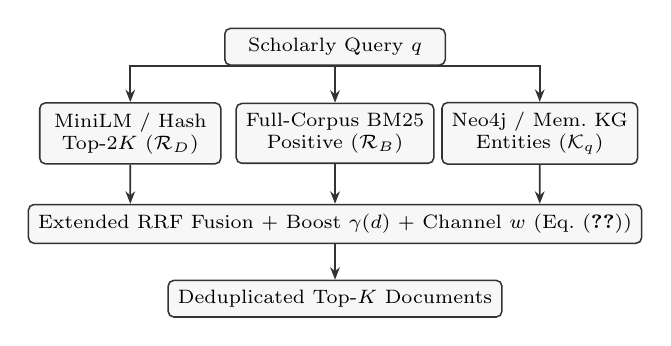
\begin{tikzpicture}
  \node[box, minimum width=2.8cm] (q) at (0, 0) {Scholarly Query $q$};
  \node[box, minimum width=2.3cm] (dense) at (-2.6, -1.1) {MiniLM / Hash\\Top-$2K$ ($\mathcal{R}_D$)};
  \node[box, minimum width=2.3cm] (bm25) at (0, -1.1) {Full-Corpus BM25\\Positive ($\mathcal{R}_B$)};
  \node[box, minimum width=2.3cm] (kg) at (2.6, -1.1) {Neo4j / Mem.\ KG\\Entities ($\mathcal{K}_q$)};
  \node[box, minimum width=6.6cm] (rrf) at (0, -2.25) {Extended RRF Fusion + Boost $\gamma(d)$ + Channel $w$ (Eq.~\eqref{eq:rrf_kg})};
  \node[box, minimum width=4.2cm] (out) at (0, -3.2) {Deduplicated Top-$K$ Documents};

  \draw[arr] (q.south) -| (dense.north);
  \draw[arr] (q.south) -- (bm25.north);
  \draw[arr] (q.south) -| (kg.north);
  \draw[arr] (dense.south) -- ([xshift=-2.6cm]rrf.north);
  \draw[arr] (bm25.south) -- (rrf.north);
  \draw[arr] (kg.south) -- ([xshift=2.6cm]rrf.north);
  \draw[arr] (rrf.south) -- (out.north);
\end{tikzpicture}
\caption{Verified hybrid retrieval pipeline with full-corpus BM25 scanning and additive KG candidate-channel fusion.}
\label{fig:retrieval_pipe}
\end{figure}

\subsection{Multi-Agent State Execution and Provider Fallback}
Direct inspection of \texttt{ai-service/agents/router.py} confirms that \texttt{agent\_workflow} compiles a deterministic 13-node linear directed LangGraph topology $M = (A, T)$ executing sequentially across shared \texttt{AgentState} $S_t$ (Fig.~\ref{fig:langgraph}). Each node $a_j \in A$ applies an incremental typed transition:
\begin{equation}
a_j : S_t \longrightarrow S_{t+1}, \qquad S_{t+1} = S_t \cup \Delta S_{a_j}.
\end{equation}

\begin{figure}[t]
\centering
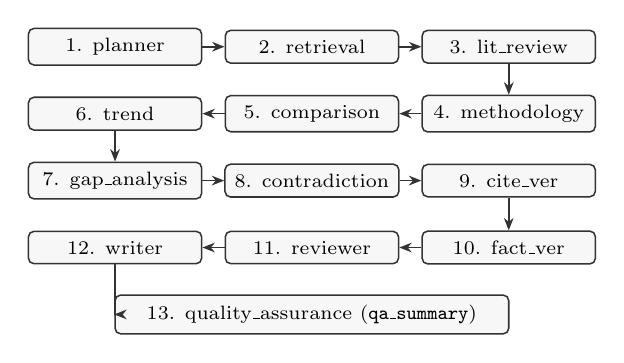
\begin{tikzpicture}
  \node[box, minimum width=2.2cm] (n1) at (-2.5, 0) {1. planner};
  \node[box, minimum width=2.2cm] (n2) at (0, 0) {2. retrieval};
  \node[box, minimum width=2.2cm] (n3) at (2.5, 0) {3. lit\_review};
  \node[box, minimum width=2.2cm] (n4) at (2.5, -0.85) {4. methodology};
  \node[box, minimum width=2.2cm] (n5) at (0, -0.85) {5. comparison};
  \node[box, minimum width=2.2cm] (n6) at (-2.5, -0.85) {6. trend};
  \node[box, minimum width=2.2cm] (n7) at (-2.5, -1.7) {7. gap\_analysis};
  \node[box, minimum width=2.2cm] (n8) at (0, -1.7) {8. contradiction};
  \node[box, minimum width=2.2cm] (n9) at (2.5, -1.7) {9. cite\_ver};
  \node[box, minimum width=2.2cm] (n10) at (2.5, -2.55) {10. fact\_ver};
  \node[box, minimum width=2.2cm] (n11) at (0, -2.55) {11. reviewer};
  \node[box, minimum width=2.2cm] (n12) at (-2.5, -2.55) {12. writer};
  \node[box, minimum width=5.0cm] (n13) at (0, -3.4) {13. quality\_assurance (\texttt{qa\_summary})};

  \draw[arr] (n1)--(n2); \draw[arr] (n2)--(n3); \draw[arr] (n3)--(n4);
  \draw[arr] (n4)--(n5); \draw[arr] (n5)--(n6); \draw[arr] (n6)--(n7);
  \draw[arr] (n7)--(n8); \draw[arr] (n8)--(n9); \draw[arr] (n9)--(n10);
  \draw[arr] (n10)--(n11); \draw[arr] (n11)--(n12);
  \draw[arr] (n12.south) |- (n13.west);
\end{tikzpicture}
\caption{Exact compiled 13-node linear LangGraph sequence verified in \texttt{ai-service/agents/router.py}.}
\label{fig:langgraph}
\end{figure}

\subsubsection{Fallback-Resilient Model Dispatch}
Agent role configurations assign task-tuned temperatures (\texttt{AGENT\_TEMPERATURES} spanning $T{=}0.0$ for verification to $T{=}0.6$ for writing) primarily via \texttt{groq/llama-3.3-70b-versatile}, backed by exponential backoff and standardized Gemini targets updated to \texttt{gemini-2.5-flash} alongside deterministic offline fallbacks when credentials are absent or rate-limited.

\subsection{Numeric-Consistent Hybrid Claim Grounding Formalism}
Resolving the legacy \texttt{verify\_claim()} defect that returned \texttt{verified} whenever non-empty evidence existed, \texttt{score\_claim\_against\_evidence()} pairs atomic claim $c$ against candidate chunk $e$ using stopword-filtered unigram coverage $J_1(c, e)$, bigram coverage $J_2(c, e)$, and optional normalized \texttt{all-MiniLM-L6-v2} cosine similarity $s_{\text{sem}}(c, e) \in [0, 1]$:
\begin{equation}
s_{\text{base}}(c, e) =
\begin{cases}
0.50\,s_{\text{sem}} + 0.35\,J_1 + 0.15\,J_2, & \text{if MiniLM loaded},\\
0.70\,J_1 + 0.30\,J_2, & \text{lexical fallback}.
\end{cases}
\end{equation}
Signed numerical values $\mathcal{N}(c)$ and $\mathcal{N}(e)$ are extracted and matched under $5\%$ relative tolerance ($N_{\text{match}}$), while sign reversals or $>10\%$ discrepancies increment $N_{\text{conflict}}$. Deterministic grading assigns:
\begin{equation}
\text{Verdict}(c, e) =
\begin{cases}
\texttt{REFUTED}, & N_{\text{conflict}} > 0 \land N_{\text{match}} = 0 \land s_{\text{base}} \ge 0.20,\\
\texttt{SUPPORTED}, & s_{\text{base}} \ge \tau_{\text{supp}} \land \neg\text{conflict\_dominant},\\
\texttt{UNVERIFIED}, & \text{otherwise},
\end{cases}
\end{equation}
with $\tau_{\text{supp}} = 0.42$ (hybrid) or $0.35$ (lexical). Post-draft auditing in \texttt{qa\_node} runs \texttt{verify\_section\_claims()} across drafted text and stores structured counts inside \texttt{final\_output["qa\_summary"]}.

\subsection{Multi-Scale Academic Integrity Formalism}
The Express integrity engine (\texttt{server/src/utils/plagiarismEngine.ts}) combines lexical, positional, structural, bibliographic, semantic, and statistical signals across project papers (\texttt{localPapers}) with optional external API skips (\texttt{\{skipExternalLookup\}}):

\begin{figure}[t]
\centering
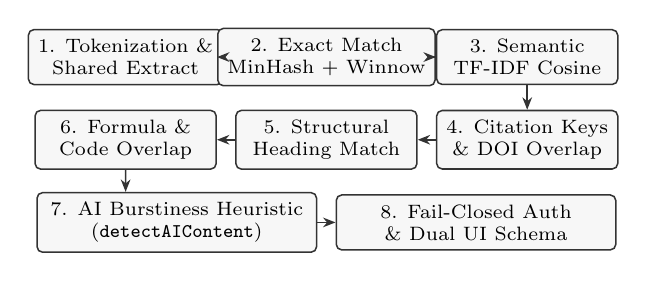
\begin{tikzpicture}
  \node[box, minimum width=2.3cm] (p1) at (-2.55, 0) {1. Tokenization \&\\Shared Extract};
  \node[box, minimum width=2.3cm] (p2) at (0, 0) {2. Exact Match\\MinHash + Winnow};
  \node[box, minimum width=2.3cm] (p3) at (2.55, 0) {3. Semantic\\TF-IDF Cosine};
  \node[box, minimum width=2.3cm] (p4) at (2.55, -1.05) {4. Citation Keys\\\& DOI Overlap};
  \node[box, minimum width=2.3cm] (p5) at (0, -1.05) {5. Structural\\Heading Match};
  \node[box, minimum width=2.3cm] (p6) at (-2.55, -1.05) {6. Formula \&\\Code Overlap};
  \node[box, minimum width=3.55cm] (p7) at (-1.9, -2.1) {7. AI Burstiness Heuristic\\(\texttt{detectAIContent})};
  \node[box, minimum width=3.55cm] (p8) at (1.9, -2.1) {8. Fail-Closed Auth\\\& Dual UI Schema};

  \draw[arr] (p1)--(p2); \draw[arr] (p2)--(p3); \draw[arr] (p3)--(p4);
  \draw[arr] (p4)--(p5); \draw[arr] (p5)--(p6);
  \draw[arr] (p6.south) -- ([xshift=-0.65cm]p7.north);
  \draw[arr] (p7)--(p8);
\end{tikzpicture}
\caption{Verified Express academic integrity pipeline unifying MinHash, Winnowing ($w{=}4$, five-token shingles), and shared structural extractors.}
\label{fig:integrity_pipe}
\end{figure}

\subsubsection{Winnowing and MinHash Fusion}
Normalized word streams are decomposed into overlapping five-token shingles (\texttt{SHINGLE\_SIZE = 5}). MinHash constructs $M{=}128$ permutation signatures (\texttt{MINHASH\_PERMUTATIONS = 128}) for global Jaccard estimation $\hat{J}(D_1, D_2) = \frac{1}{M}\sum_{m=1}^{M}\mathbb{I}[\text{sig}_m(D_1){=}\text{sig}_m(D_2)]$. Concurrently, \texttt{winnowingFingerprint()} slides a window of size $w{=}4$ (\texttt{windowSize = 4}) across hashed five-token shingles, selecting the rightmost minimum fingerprint per window. Unifying previously disconnected code paths, \texttt{detectExactPlagiarism()} evaluates
\begin{equation}
S_{\text{exact}} = \max\!\big(\hat{J}_{\text{MinHash}},\, J_{\text{Winnow}}\big),
\end{equation}
augmented by a short-sentence overlap floor to capture localized patchwrites inside multi-paragraph submissions.

\subsubsection{Shared Structural, Formula, and Code Extraction}
Extracting a common helper \texttt{extractStructuralElementsFromText()} parses Markdown section headers, inline/display LaTeX expressions (\texttt{\$...\$/\$\$...\$\$}), and fenced code listings uniformly for both query documents and \texttt{localPapers}, eliminating prior zeroed structural scores caused by unpopulated reference fields.

\subsubsection{AI-Content Detection Heuristics}
Heuristic AI analysis in \texttt{detectAIContent()} evaluates sentence-length burstiness (coefficient of variation $\sigma_L / \mu_L$ over sentence lengths $L{=}\{l_1,\dots,l_S\}$) alongside repetitive formal-transition counters, yielding a continuous \texttt{aiProbability} evaluated against a default 50\% flagging cutoff.

\section{System Architecture and Implementation}
ResearcherGPT spans Python retrieval/orchestration services, Express integrity/auth middleware, and Next.js presentation modules verified cleanly on the \texttt{research-validation} branch.

\subsection{Tri-Hybrid Retrieval with KG Channel Injection}
Algorithm~\ref{alg:hybrid_kg} details \texttt{retrieve\_hybrid()} in \texttt{ai-service/rag/hybrid\_retriever.py}. All three candidate channels are deduplicated by document identifier prior to scoring via Eq.~\eqref{eq:rrf_kg}.

\begin{algorithm}[t]
\caption{Full-Corpus Hybrid RRF with KG Channel (\texttt{hybrid\_retriever.py})}
\label{alg:hybrid_kg}
\footnotesize
\begin{algorithmic}[1]
\Require Project ID $p$, query $q$, limit $K$, boost $\beta{=}1.30$, channel $w$
\Ensure Top-$K$ unique ranked documents $\mathcal{R}_K$
\State $\hat{q} \gets \text{EncodeQuery}(q)$ \Comment{MiniLM-L6-v2 or 384-d \texttt{blake2b}}
\State $\mathcal{R}_D \gets \text{SearchRelevantChunks}(\hat{q}, p, 2K)$
\State $\mathcal{C}_p \gets \text{ScrollProjectChunks}(p)$ \Comment{Full project corpus}
\State $\mathcal{R}_B \gets \{c \in \text{BM25}(q, \mathcal{C}_p, 2K) : \text{score}(c) > 0\}$
\State $W_q \gets \text{ExtractTokens}(q, \text{minlen} \ge 4)$
\State $\mathcal{K}_q \gets \text{QueryKnowledgeGraph}(W_q, p)$ \Comment{By entity hits}
\State Deduplicate $\mathcal{R}_D, \mathcal{R}_B$ to 1-based paper ranks $r_D, r_B$
\State $\mathcal{U} \gets \text{Papers}(\mathcal{R}_D) \cup \text{Papers}(\mathcal{R}_B)$
\If{$w > 0$}
  \State $\mathcal{U} \gets \mathcal{U} \cup \mathcal{K}_q$ \Comment{Eliminate multi-hop starvation}
\EndIf
\ForAll{$d \in \mathcal{U}$}
  \State Compute $S_{\text{RRF+KG}}(d)$ via Eq.~\eqref{eq:rrf_kg}
\EndFor
\State \Return $\text{TopK}(\mathcal{U}, S_{\text{RRF+KG}}, K)$
\end{algorithmic}
\end{algorithm}

\subsection{Thirteen Compiled Cognitive Agents}
Table~\ref{tab:agents} specifies the exact 13 compiled nodes registered in \texttt{ai-service/agents/router.py} alongside verified \texttt{AGENT\_TEMPERATURES} and responsibilities.

\begin{table*}[t]
\centering
\caption{Verified Agent Specifications in Compiled Linear LangGraph Topology (\texttt{router.py})}
\label{tab:agents}
\footnotesize
\setlength{\tabcolsep}{4pt}
\begin{tabular}{rllcp{7.2cm}}
\toprule
\textbf{No.} & \textbf{Node ID} & \textbf{Primary Config Target} & \textbf{Temp.} & \textbf{Verified Operational Responsibility} \\
\midrule
1 & \texttt{planner} & \texttt{groq/llama-3.3-70b-versatile} & 0.3 & Entry node; decomposes research question into structured sub-queries \\
2 & \texttt{retrieval} & \texttt{researcher} (\texttt{llama-3.3-70b}) & --- & Executes dense, full-corpus BM25, and KG candidate-channel search \\
3 & \texttt{literature\_review} & \texttt{groq/llama-3.3-70b-versatile} & 0.4 & Aggregates authors, architectures, datasets, and empirical context \\
4 & \texttt{methodology\_extraction} & \texttt{groq/llama-3.3-70b-versatile} & 0.2 & Extracts formal procedures, hyperparameters, and model settings \\
5 & \texttt{comparison} & \texttt{groq/llama-3.3-70b-versatile} & 0.2 & Synthesizes comparative matrices across retrieved baselines \\
6 & \texttt{trend\_analysis} & \texttt{groq/llama-3.3-70b-versatile} & 0.5 & Analyzes chronological evolution across reviewed works \\
7 & \texttt{gap\_analysis} & \texttt{groq/llama-3.3-70b-versatile} & 0.3 & Identifies methodological deficiencies and open dataset gaps \\
8 & \texttt{contradiction} & \texttt{groq/llama-3.3-70b-versatile} & 0.1 & Mines empirical conflicts and divergent quantitative claims \\
9 & \texttt{citation\_verification} & \texttt{gemini-2.5-flash} / local check & 0.0 & Cross-checks inline bracketed references against source paper IDs \\
10 & \texttt{fact\_verification} & \texttt{groq/llama-3.3-70b-versatile} & 0.0 & Validates atomic propositions against top retrieved chunks \\
11 & \texttt{reviewer} & \texttt{groq/llama-3.3-70b-versatile} & 0.3 & Simulates conference-style critique of synthesized manuscript sections \\
12 & \texttt{writer} & \texttt{groq/llama-3.3-70b-versatile} & 0.6 & Compiles academic section drafts and formatted LaTeX prose \\
13 & \texttt{quality\_assurance} & \texttt{qa\_node} + \texttt{verify\_section\_claims} & 0.1 & Audits claim veracity and reference validity into \texttt{qa\_summary} \\
\bottomrule
\end{tabular}
\end{table*}

\subsection{Fact Verification Engine}
Algorithm~\ref{alg:claim_audit} documents \texttt{verify\_section\_claims()} invoked by terminal node \texttt{quality\_assurance}. Running deterministically offline under \texttt{allow\_llm=False} eliminates silent pass-through support while remaining extensible to online \texttt{gemini-2.5-flash} tie-breaking.

\begin{algorithm}[t]
\caption{Post-Draft Claim and Citation Audit (\texttt{claim\_verifier.py})}
\label{alg:claim_audit}
\footnotesize
\begin{algorithmic}[1]
\Require Draft text $T_{\text{sec}}$, project $p$, valid refs $\mathcal{V}_{\text{ref}}$, flag \texttt{allow\_llm}
\Ensure QA report dictionary $Q_{\text{audit}}$
\State $\mathcal{A} \gets \text{SplitClaims}(T_{\text{sec}})$
\State Check bracketed citations $\mathcal{B}_{\text{cite}}$ against $\mathcal{V}_{\text{ref}}$
\ForAll{$c \in \mathcal{A}$}
  \State $\mathcal{E}_c \gets \text{SearchRelevantChunks}(c, p, \text{top\_k}{=}3)$
  \State $(s_{\text{base}}, N_{\text{match}}, N_{\text{conflict}}) \gets \text{ScoreClaim}(c, \mathcal{E}_c)$
  \If{\texttt{allow\_llm} and borderline score}
    \State Consult \texttt{gemini-2.5-flash} audit tie-breaker
  \EndIf
  \State Classify $c \in \{\texttt{SUPPORTED}, \texttt{REFUTED}, \texttt{UNVERIFIED}\}$
\EndFor
\State \Return Counts, per-claim provenance, and citation validity rate
\end{algorithmic}
\end{algorithm}

\subsection{FormaTeX Layout Compilation and Security Hardening}
In \texttt{pdf\_processor.py}, \texttt{extract\_pdf\_content()} preserves reading order with PyMuPDF, extracts DOI identifiers via regex, attaches explicit \texttt{chunk\_index} metadata, and calls \texttt{extract\_tables\_with\_pdfplumber()} to recover 2D ruled tables. Prior to compilation, \texttt{PaperValidator.sanitize\_paper\_structure()} normalizes headings to Roman-numeral IEEE conventions and deduplicates references. For remote rendering, \texttt{FormaTeXService} targets multi-style templates while loading \texttt{FORMATEX\_API\_KEY} strictly from environment variables (with hardcoded secret literals removed) and embedding referenced local images via base64 encoding. Target template classes mapped across downstream exporters include:
\begin{itemize}
  \item \emph{IEEE:} \texttt{\textbackslash documentclass[conference]\{IEEEtran\}} two-column layout with IEEE-style numbered references.
  \item \emph{ACM:} \texttt{\textbackslash documentclass[sigconf]\{acmart\}} with ACM metadata.
  \item \emph{Springer:} \texttt{\textbackslash documentclass[sn-mathphys,iicol]\{sn-jnl\}}.
  \item \emph{Elsevier:} \texttt{\textbackslash documentclass[review,3p,times]\{elsarticle\}}.
\end{itemize}
In parallel, \texttt{server/src/middlewares/auth.middleware.ts} enforces fail-closed \texttt{401 Unauthorized} responses in \texttt{NODE\_ENV=production} unless \texttt{ALLOW\_DEV\_MOCK\_AUTH=true}, while \texttt{client/src/app/plagiarism/page.tsx} normalizes Express and Python report payloads seamlessly.

\section{Results and Discussion}
\label{sec:results}

\subsection{Experimental Setup and Benchmark Corpus}
To establish reproducible, statistically grounded evidence isolated from API rate limits and network latency, all five evaluation suites under \texttt{evaluation/} execute offline with fixed seed \texttt{42}, local Qdrant/Neo4j fallbacks, \texttt{allow\_llm=False} for claim scoring, and \texttt{\{skipExternalLookup: true\}} for Express integrity tests. All evaluation benchmarks are disjoint from the Python and TypeScript regression unit tests. Continuous and bounded discrete metrics report two-sided 95\% percentile confidence intervals from $B{=}2{,}000$ bootstrap resamples via \texttt{evaluation/stats/stats\_utils.py}, while paired retrieval comparisons across all $N{=}75$ queries report two-sided Wilcoxon signed-rank and 5,000-resample paired permutation $p$-values (\texttt{perm\_p}). Note that offline execution left cross-encoder weights uncached in \texttt{reranker.py}, isolating retriever and KG channel contributions cleanly. Table~\ref{tab:retrieval_configs} summarizes the nine retrieval configurations tested across 60 documents (180 chunks) and 75 stratified queries (25 \texttt{lexical\_identifier}, 25 \texttt{semantic\_paraphrase}, 25 \texttt{multihop\_kg}).

\begin{table}[t]
\centering
\caption{Retrieval Ablation Configurations ($N{=}75$ Queries)}
\label{tab:retrieval_configs}
\footnotesize
\setlength{\tabcolsep}{4pt}
\begin{tabular}{lp{3.7cm}cc}
\toprule
\textbf{ID} & \textbf{Encoder / Sparse Configuration} & $\beta$ & \textbf{Ch.\ $w$} \\
\midrule
M0 & 384-d \texttt{blake2b} signed hash dense only & 1.00 & 0.00 \\
M1 & \texttt{all-MiniLM-L6-v2} dense only & 1.00 & 0.00 \\
M2 & Full-corpus BM25 only (180 chunks) & 1.00 & 0.00 \\
M3 & Pre-fix CR-1 (BM25 on dense top-$2k$) & 1.00 & 0.00 \\
M4 & Fixed full-corpus hybrid (no KG) & 1.00 & 0.00 \\
M5 & Fixed hybrid + multiplicative KG only & 1.30 & 0.00 \\
M6 & Fixed hybrid + KG channel ($w{=}0.50$) & 1.30 & 0.50 \\
\textbf{M7} & \textbf{Fixed hybrid + KG channel (Default)} & \textbf{1.30} & \textbf{0.75} \\
\textbf{M8} & \textbf{Fixed hybrid + KG channel (Equal)} & \textbf{1.30} & \textbf{1.00} \\
\bottomrule
\end{tabular}
\end{table}

\subsection{Retrieval Efficacy and Rank-Fusion Precision (RQ1)}
Offline indexing of 180 chunks took 0.032~s with signed hashing versus 119.751~s with CPU \texttt{all-MiniLM-L6-v2}. Table~\ref{tab:retrieval_results} and Fig.~\ref{fig:retrieval} report complete metrics and stratum scores:
\begin{itemize}
  \item \emph{Complementary single-mode regimes:} \texttt{M2} BM25 achieves 1.000 Recall@5 and 1.000 MRR on \texttt{lexical\_identifier} (3.82~ms/query) but scores 0.000 on paraphrases and multi-hop queries. Conversely, \texttt{M1} MiniLM achieves 1.000 on \texttt{semantic\_paraphrase} (34.14~ms) but drops to 0.613 MRR on exact identifiers, while signed hashing \texttt{M0} preserves exact identifiers (1.000 MRR, 6.35~ms) with 0.080 paraphrase recall.
  \item \emph{Full-corpus CR-1 improvement:} Fixing sub-corpus BM25 starvation (\texttt{M3} $\rightarrow$ \texttt{M4}) raises \texttt{lexical\_identifier} MRR from 0.657 to \textbf{0.833} and overall \texttt{Hit@1} from 0.467 to 0.520.
  \item \emph{KG candidate-channel efficacy:} Pure multiplicative boosting (\texttt{M5}) hits a 0.180 ceiling on multi-hop Recall@5, and sub-threshold $w{=}0.50$ (\texttt{M6}) remains tied at 0.180. Above threshold, deployed default \texttt{M7 ($w{=}0.75$)} elevates overall Recall@5 to \textbf{0.760} (multi-hop 0.280, MRR 0.740; Wilcoxon $p{=}0.000911$, $\text{perm\_p}{=}0.0004$ vs.\ \texttt{M3}; $p{=}0.000526$ vs.\ \texttt{M1} MRR). Equal-weight \texttt{M8 ($w{=}1.00$)} reaches \textbf{0.840} Recall@5 (MRR \textbf{0.782}, nDCG@5 \textbf{0.768}, multi-hop Recall@5 \textbf{0.520}, multi-hop MRR \textbf{0.600}; Wilcoxon $p{=}0.000290$ vs.\ \texttt{M3}; $p{=}8.7\times 10^{-5}$ vs.\ \texttt{M1} MRR) at 38.17~ms/query while holding lexical MRR at 0.833 and semantic Recall@5 at 1.000, supporting \textbf{H1}.
\end{itemize}

\begin{table*}[t]
\centering
\caption{Retrieval Ablation Performance ($N{=}75$ Queries, 60 Documents / 180 Chunks, 2,000-Resample 95\% Bootstrap CIs)}
\label{tab:retrieval_results}
\footnotesize
\setlength{\tabcolsep}{4.5pt}
\begin{tabular}{lccccccc}
\toprule
\textbf{Strategy} & \textbf{Recall@5 [95\% CI]} & \textbf{Hit@1} & \textbf{MRR} & \textbf{nDCG@5} & \textbf{Lex.\ MRR} & \textbf{Sem.\ R@5} & \textbf{Multi-Hop R@5 (MRR)} \\
\midrule
M0 Hash Dense Only & 0.360 [0.253, 0.467] & 0.333 & 0.340 & 0.345 & 1.000 & 0.080 & 0.000 (0.000) \\
M2 BM25 Full Corpus & 0.333 [0.227, 0.440] & 0.333 & 0.333 & 0.333 & 1.000 & 0.000 & 0.000 (0.000) \\
M1 MiniLM Dense Only & 0.653 [0.547, 0.760] & 0.467 & 0.562 & 0.580 & 0.613 & 1.000 & 0.080 (0.071) \\
M3 CR-1 Buggy Hybrid & 0.687 [0.580, 0.787] & 0.467 & 0.573 & 0.598 & 0.657 & 1.000 & 0.060 (0.063) \\
M4 Fixed Hybrid ($\beta{=}1$) & 0.673 [0.567, 0.780] & 0.520 & 0.596 & 0.612 & 0.833 & 1.000 & 0.020 (0.040) \\
M5 KG Mult.\ Only ($\beta{=}1.3$) & 0.727 [0.627, 0.820] & 0.627 & 0.702 & 0.678 & 0.833 & 1.000 & 0.180 (0.360) \\
M6 KG Channel ($w{=}0.50$) & 0.727 [0.627, 0.820] & 0.613 & 0.696 & 0.675 & 0.833 & 1.000 & 0.180 (0.340) \\
\textbf{M7 KG Channel ($w{=}0.75$)} & \textbf{0.760 [0.673, 0.847]} & \textbf{0.640} & \textbf{0.740} & \textbf{0.705} & \textbf{0.833} & \textbf{1.000} & \textbf{0.280 (0.473)} \\
\textbf{M8 KG Channel ($w{=}1.00$)} & \textbf{0.840 [0.760, 0.913]} & \textbf{0.680} & \textbf{0.782} & \textbf{0.768} & \textbf{0.833} & \textbf{1.000} & \textbf{0.520 (0.600)} \\
\bottomrule
\end{tabular}
\end{table*}

\begin{figure}[t]
  \centering
  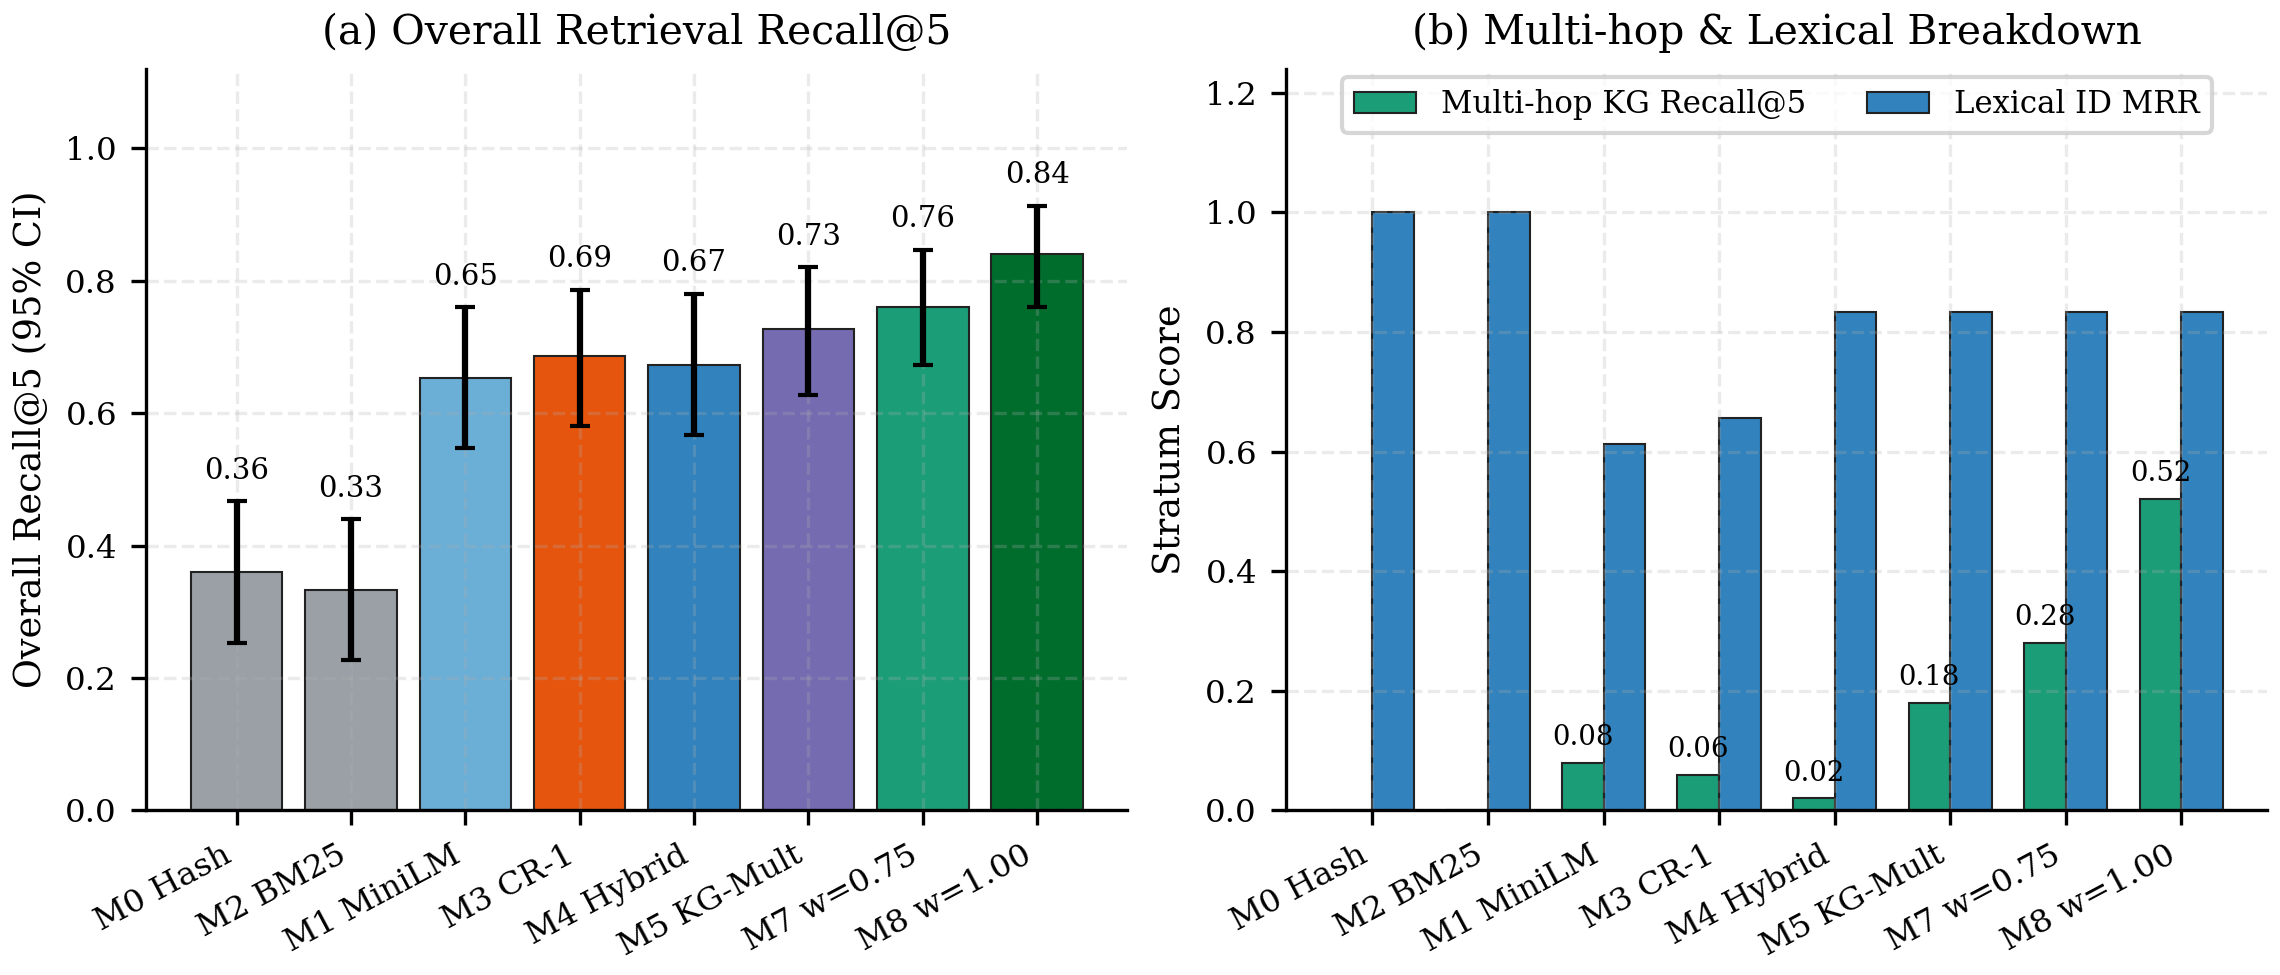
\includegraphics[width=\columnwidth]{figures/retrieval_ablation.png}
  \caption{(a) Overall Recall@5 with 95\% bootstrap CIs across retrieval configurations; (b) Multi-hop KG Recall@5 versus Lexical-ID MRR confirming multi-hop recovery without single-hop lexical regression.}
  \label{fig:retrieval}
\end{figure}

\subsection{Factual Grounding and Citation Accuracy (RQ2)}
Across 90 balanced claims (Table~\ref{tab:grounding} and Fig.~\ref{fig:grounding_integrity}(a)), legacy \texttt{V0} exhibits \texttt{FPR = 1.000} (3-way accuracy 0.667) because any evidence yields acceptance. Lexical+numeric verifier \texttt{V1} cuts false support to \texttt{FPR = 0.000} (precision 1.000, F1 0.966, 3-way accuracy \textbf{0.900} [0.833, 0.956]) in 0.065~ms/claim. Hybrid MiniLM+numeric verifier \texttt{V2} lifts binary recall to 1.000, binary accuracy to \textbf{0.989}, F1 to \textbf{0.992}, and 3-way accuracy to \textbf{0.944} [0.889, 0.989] (\texttt{FPR = 0.033}, 44.99~ms/claim), confirming \textbf{H2}. Both \texttt{V1} and \texttt{V2} attain \textbf{0.667} numeric refutation recall; the remaining third with sparse lexical context falls conservatively into \texttt{UNVERIFIED}. End-to-end auditing of a 4-claim drafted sample via \texttt{verify\_section\_claims()} returned exact counts: \texttt{2} verified, \texttt{1} refuted, \texttt{1} unverified, and \texttt{3/4} valid citations (\texttt{0.750}).

\begin{table}[t]
\centering
\caption{Factual Grounding Results ($N{=}90$ Balanced Claims)}
\label{tab:grounding}
\footnotesize
\setlength{\tabcolsep}{3pt}
\begin{tabular}{lccccc}
\toprule
\textbf{Verifier} & \textbf{Acc.} & \textbf{F1} & \textbf{FPR} & \textbf{3-Way [95\% CI]} & \textbf{ms} \\
\midrule
V0 Legacy & 0.667 & 0.800 & 1.000 & 0.667 [0.567, 0.767] & 0.0003 \\
V1 Lex+Num & 0.956 & 0.966 & 0.000 & 0.900 [0.833, 0.956] & 0.0649 \\
\textbf{V2 Hybrid} & \textbf{0.989} & \textbf{0.992} & \textbf{0.033} & \textbf{0.944 [0.889, 0.989]} & 44.99 \\
\bottomrule
\end{tabular}
\end{table}

\begin{figure}[t]
  \centering
  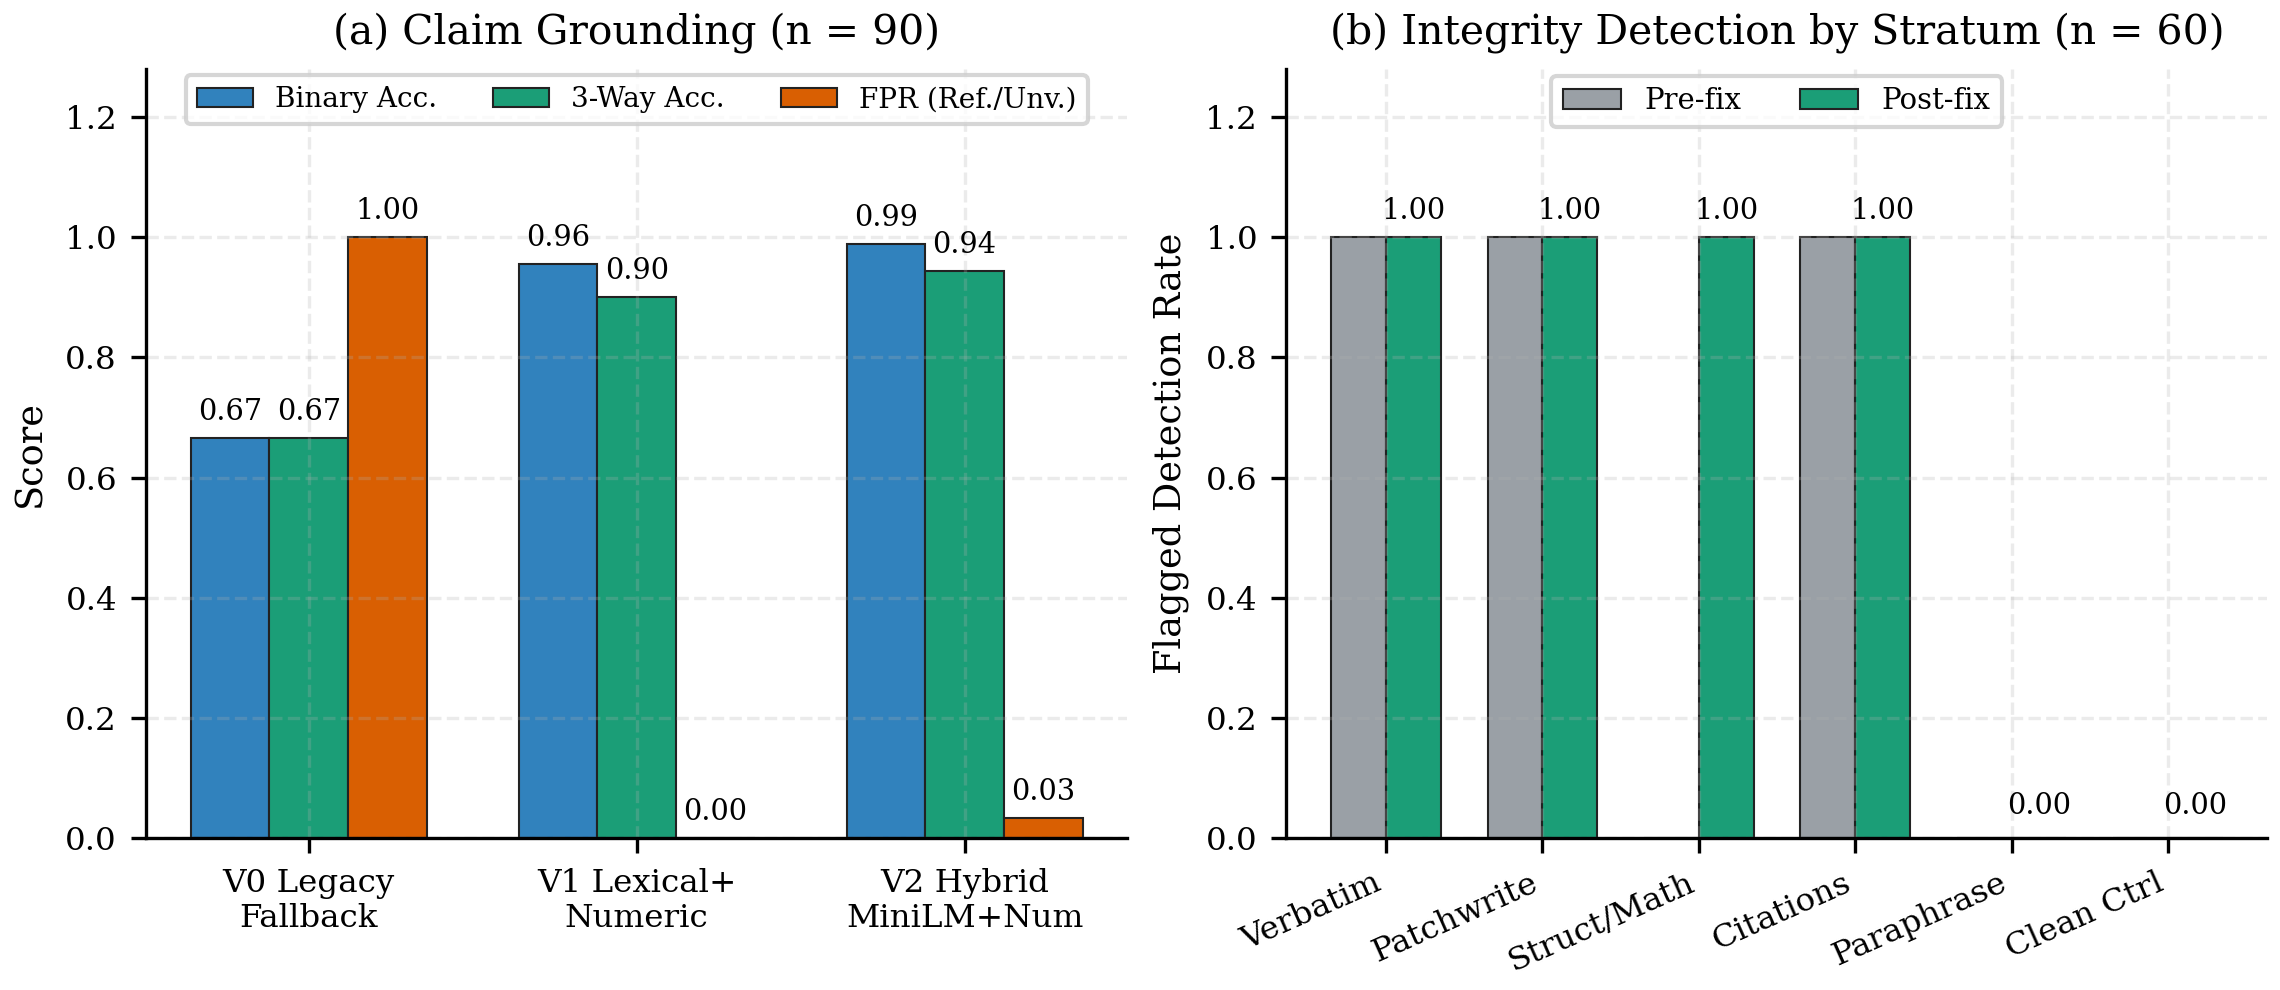
\includegraphics[width=\columnwidth]{figures/grounding_and_integrity.png}
  \caption{(a) Claim grounding performance on $n{=}90$ claims comparing \texttt{V0}, \texttt{V1}, and \texttt{V2}; (b) Plagiarism detection rate pre-fix vs.\ post-fix across six integrity strata ($n{=}60$).}
  \label{fig:grounding_integrity}
\end{figure}

\subsection{Plagiarism and Attribution Engine Performance (RQ3)}
Evaluated over 60 controlled integrity pairs (3.44~ms/pair, 95\% CI [3.08, 3.98]), wiring Winnowing and shared \texttt{extractStructuralElementsFromText()} lifts overall recall from 0.600 to \textbf{0.800}, F1 from 0.750 to \textbf{0.889}, and accuracy from 0.667 to \textbf{0.833} at \textbf{1.000} precision and \textbf{0.000} false positives on clean controls (Table~\ref{tab:integrity} and Fig.~\ref{fig:grounding_integrity}(b)). Notably, \texttt{structure\_formula\_code} improves from \textbf{0.000} to \textbf{1.000} (\texttt{score=100} across headings, LaTeX, and code), partially confirming \textbf{H3}. However, TypeScript \texttt{semantic\_paraphrase} remains at \textbf{0.000} due to sparse TF-IDF bag-of-words limits, and on 30 synthetic AI/human texts \texttt{detectAIContent()} produces clean mean score separation (\texttt{35.0} vs.\ \texttt{0.0}) yet \texttt{0.000} recall against its uncalibrated 50\% threshold.

\begin{table}[t]
\centering
\caption{Integrity Engine Pre-Fix vs.\ Post-Fix ($N{=}60$) and AI Heuristic ($N{=}30$)}
\label{tab:integrity}
\footnotesize
\setlength{\tabcolsep}{4pt}
\begin{tabular}{p{4.3cm}cc}
\toprule
\textbf{Metric / Test Category} & \textbf{Pre-Fix} & \textbf{Post-Fix} \\
\midrule
Overall Precision / FPR & 1.000 / 0.000 & 1.000 / 0.000 \\
Overall Recall / F1 & 0.600 / 0.750 & \textbf{0.800 / 0.889} \\
Overall Accuracy & 0.667 & \textbf{0.833} \\
\midrule
\texttt{verbatim\_exact} ($n{=}10$, score 75) & 1.000 & 1.000 \\
\texttt{localized\_patchwrite} ($n{=}10$, score 38) & 1.000 & 1.000 \\
\texttt{structure\_formula\_code} ($n{=}10$) & 0.000 & \textbf{1.000} \\
\texttt{citation\_overlap} ($n{=}10$, score 10) & 1.000 & 1.000 \\
\texttt{semantic\_paraphrase} ($n{=}10$) & 0.000 & 0.000 \\
\texttt{clean\_negative\_control} ($n{=}10$) & 0.000 & 0.000 \\
\midrule
AI Heuristic Recall@50\% (AI vs.\ Human mean) & \multicolumn{2}{c}{0.000 (35.0 vs.\ 0.0)} \\
\bottomrule
\end{tabular}
\end{table}

\subsection{Document Extraction and Offline Graph Execution (RQ4)}
Across 15 synthetic two-column PDFs (Table~\ref{tab:extraction_orch}), \texttt{extract\_pdf\_content()} recovered 1.000 planted tokens and 1.000 DOIs, while \texttt{extract\_tables\_with\_pdfplumber()} lifted ruled-table recall from 0.000 to \textbf{1.000} (\texttt{1.000} exact cell-row match) in 74.88~ms/PDF ([59.55, 101.97]), supporting \textbf{H4}. On an actual 11-page prototype manuscript PDF, ingestion produced 61 chunks and 1 table in 2,150.63~ms, and \texttt{PaperValidator} normalized mixed headings and deduplicated references from 3 to 2. Across 5 offline runs, all 13 compiled LangGraph nodes finished in 138.10~ms ([104.72, 190.62]) using 0.295~MB peak heap (\texttt{1.000} mock citation validity; \texttt{0.000} claim support because deterministic mock text omits planted numeric assertions).

\begin{table}[t]
\centering
\caption{PDF Extraction ($N{=}15$ + Real Artifact) and Offline Graph Execution ($N{=}5$)}
\label{tab:extraction_orch}
\footnotesize
\setlength{\tabcolsep}{4pt}
\begin{tabular}{p{4.6cm}c}
\toprule
\textbf{Subsystem Metric} & \textbf{Value [95\% CI]} \\
\midrule
Synthetic PDF Token Recall & 1.000 [1.000, 1.000] \\
Synthetic PDF DOI Exact Match & 1.000 [1.000, 1.000] \\
Table Recall: Text $\rightarrow$ \texttt{pdfplumber} & 0.000 $\rightarrow$ \textbf{1.000} [1.000, 1.000] \\
\texttt{pdfplumber} Exact Row Match & 1.000 [1.000, 1.000] \\
Synthetic PDF Latency (ms) & 74.88 [59.55, 101.97] \\
11-Page PDF (Chunks / Tables / ms) & 61 / 1 / 2150.63 \\
\midrule
Compiled 13-Node Completion Rate & 1.000 \\
Offline Graph Latency (ms) & 138.10 [104.72, 190.62] \\
Peak Traced Heap (MB) & 0.295 [0.198, 0.477] \\
\bottomrule
\end{tabular}
\end{table}

\subsection{Regression Verification and Security Hygiene}
All automated regression checks pass after final fixes:
\begin{itemize}
  \item \emph{Python regressions (\texttt{test\_phase1\_regressions.py}):} 8/8 unit tests passed (0.598~s), verifying BM25 punctuation tokenization, numeric refutation, post-draft QA emission, feature hashing similarity, \texttt{FORMATEX\_API\_KEY} env loading, full-corpus CR-1 recovery, in-memory KG boost, \texttt{pdfplumber} tables, and \texttt{chunk\_index} metadata.
  \item \emph{TypeScript/Next.js builds \& integrity tests (\texttt{phase1Regressions.unit.ts}):} Server and client \texttt{tsc --noEmit} and server \texttt{npm run build} exited \texttt{0}; Express tests printed \texttt{ALL SERVER PHASE 1 UNIT TESTS PASSED}, confirming Winnowing, non-zero structural/formula/code/citation overlap, and production \texttt{401} auth gating.
  \item \emph{LaTeX audit (\texttt{validate\_latex.py}):} Verified zero syntax/escaping/environment/reference defects.
\end{itemize}

\subsection{Limitations and Threats to Validity}
Four explicit boundaries govern external generalization:
\begin{enumerate}
  \item \emph{Remaining multi-hop surface-label misses (48\% at $w{=}1.00$):} Literal label matching in \texttt{query\_papers\_by\_terms()} misses abstract bridge concepts absent from indexed entity text.
  \item \emph{Sparse semantic paraphrase gap in Express:} Heavy lexical rewrites evade sparse TF-IDF cosine in TypeScript (\texttt{0.000}), requiring optional forwarding to Python \texttt{all-MiniLM-L6-v2}.
  \item \emph{Conservative AI detector threshold:} Separating \texttt{35.0} vs.\ \texttt{0.0} probabilities yields zero hits at fixed 50\% flagging cutoff until ROC calibration is learned over open corpora.
  \item \emph{Offline scope vs.\ external infrastructure:} Curated offline suites isolate mechanisms rigorously but exclude live Gemini 2.5 inference latency, remote Qdrant/Neo4j scaling, public BEIR/SciFact benchmarks, Clerk JWKS verification, and remote FormaTeX PDF rendering.
\end{enumerate}

\subsection{Extended Technical Roadmap (Proposed Extensions)}
Distinct from deployed behavior validated above, we specify six concrete engineering extensions proposed for subsequent development cycles: (1) synonym expansion and cached cross-encoder reranking inside \texttt{reranker.py}; (2) asynchronous MiniLM paraphrase forwarding from Express; (3) cost-aware adaptive routing replacing static linear LangGraph edges; (4) kernel-checked mathematical verification via Lean~4/Mathlib; (5) streaming OpenAlex provenance ingestion; and (6) sandboxed execution of manuscript code snippets.

\section{Conclusion and Future Work}

\subsection{Comprehensive Synthesis and Retrospective Conclusion}
We audited, hardened, and empirically evaluated \emph{ResearcherGPT} across full-corpus hybrid retrieval, numeric-consistent claim verification, layout-aware PDF table parsing, multi-scale plagiarism analysis, and 13-node LangGraph execution. Eliminating sub-corpus BM25 starvation (\texttt{CR-1}) and introducing additive KG candidate-channel RRF fusion raised Recall@5 to 0.760 at $w{=}0.75$ and 0.840 at $w{=}1.00$ ($p{=}0.000290$), lifting multi-hop Recall@5 to 0.520 without sacrificing exact lexical MRR (0.833) or semantic recall (1.000). Hybrid MiniLM + numeric grounding lifted 3-way claim accuracy to 0.944 with 0.033 FPR; \texttt{pdfplumber} lifted ruled-table recall to 1.000; and unified Winnowing + shared structural extraction raised integrity F1 from 0.750 to 0.889. Every empirical claim traces directly to executable code and deterministic CSV/JSON logs.

\subsection{Current System and Extended Technical Roadmap}
Fig.~\ref{fig:roadmap} and Table~\ref{tab:roadmap} contrast the verified baseline against proposed engineering extensions explicitly marked as non-deployed roadmap targets.

\begin{figure}[t]
\centering
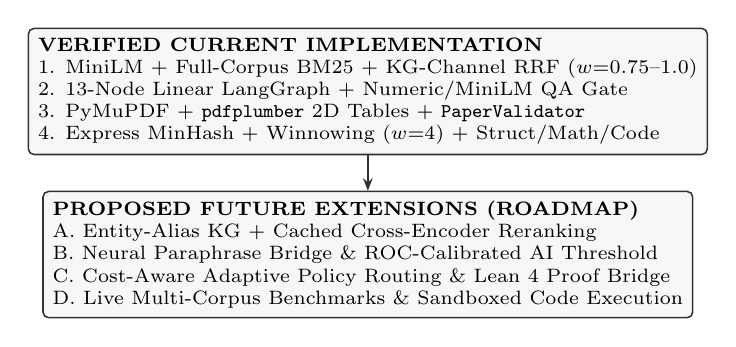
\begin{tikzpicture}[node distance=0.45cm]
  \node[box, minimum width=7.6cm, align=left] (cur) {\textbf{VERIFIED CURRENT IMPLEMENTATION}\\
  1. MiniLM + Full-Corpus BM25 + KG-Channel RRF ($w{=}0.75$--$1.0$)\\
  2. 13-Node Linear LangGraph + Numeric/MiniLM QA Gate\\
  3. PyMuPDF + \texttt{pdfplumber} 2D Tables + \texttt{PaperValidator}\\
  4. Express MinHash + Winnowing ($w{=}4$) + Struct/Math/Code};
  \node[box, minimum width=7.6cm, align=left, below=of cur] (fut) {\textbf{PROPOSED FUTURE EXTENSIONS (ROADMAP)}\\
  A. Entity-Alias KG + Cached Cross-Encoder Reranking\\
  B. Neural Paraphrase Bridge \& ROC-Calibrated AI Threshold\\
  C. Cost-Aware Adaptive Policy Routing \& Lean 4 Proof Bridge\\
  D. Live Multi-Corpus Benchmarks \& Sandboxed Code Execution};
  \draw[arr] (cur) -- (fut);
\end{tikzpicture}
\caption{Transition from code-verified ResearcherGPT baseline to proposed engineering roadmap.}
\label{fig:roadmap}
\end{figure}

\begin{table*}[t]
\centering
\caption{Technical Specification Matrix for Proposed Future Work (Not Yet Implemented)}
\label{tab:roadmap}
\footnotesize
\setlength{\tabcolsep}{4pt}
\begin{tabular}{p{2.7cm}p{3.0cm}p{4.3cm}p{4.8cm}}
\toprule
\textbf{Proposed Extension} & \textbf{Core Mechanism} & \textbf{Target Integration Point} & \textbf{Verification Target} \\
\midrule
A. Alias-Aware KG & Query alias expansion & Cached \texttt{ms-marco-MiniLM} + alias lookup & Reduce 48\% multi-hop surface misses \\
B. Paraphrase Bridge & Async neural similarity & Express $\rightarrow$ Python MiniLM endpoint & Lift TS \texttt{semantic\_paraphrase} $>0.000$ \\
C. Adaptive Routing & Constrained policy $\pi_\theta$ & Conditional review gates in \texttt{router.py} & Lower token cost per verified claim \\
D. Proof Checking & Kernel-checked Lean 4 & Post-\texttt{PaperValidator} formula pass & Verify mathematical soundness \\
E. Streaming Mesh & Time-decayed weights & BullMQ + OpenAlex event stream & Track citation retractions cleanly \\
F. Live Evaluation & BEIR/SciFact + live LLMs & Extended suites under \texttt{evaluation/} & Establish in-the-wild latency bounds \\
\bottomrule
\end{tabular}
\end{table*}

\subsection{Actionable Future Work}
\begin{enumerate}
  \item \emph{Adaptive Agent Routing:} Future policies $\pi_\theta(a_t \mid S_t)$ can select verify, loop, prune, or terminate actions maximizing claim gain $\Delta F$ minus token cost and unresolved contradiction count:
  \begin{equation}
  R(S_t, a_t) = \lambda_1\Delta F + \lambda_2\Delta C - \lambda_3\,\text{Cost}_{\text{tokens}}(a_t) - \lambda_4 I_{\text{unresolved}}.
  \end{equation}
  \item \emph{Mechanical Proof Verification:} Translating LaTeX derivations into Lean~4 / Mathlib proof obligations separates syntactic formatting from formal deductive soundness.
  \item \emph{Native Vector Diagram Compilation:} Emitting declarative TikZ/Asymptote schematics inside \texttt{FormaTeX} ensures publication font consistency across exported figures.
  \item \emph{Streaming Knowledge Mesh:} Incremental OpenAlex ingestion can weight graph edges temporally across publication age $t - t_{\text{pub}}$:
  \begin{equation}
  w(u, v, t) = w_0(u, v)\exp\!\big[-\lambda(t - t_{\text{pub}})\big].
  \end{equation}
  \item \emph{Isolated Reproducibility Sandboxes:} Bounded WebAssembly/container runners can audit empirical metric discrepancy via
  \begin{equation}
  \text{ReproScore} = 1 - \frac{|M_{\text{reported}} - M_{\text{measured}}|}{\max(|M_{\text{reported}}|, |M_{\text{measured}}|, \epsilon)},
  \end{equation}
  when benchmark definitions and inputs align strictly.
  \item \emph{Public Live Benchmarks:} Extending offline suites onto open scholarly datasets (SciFact/BEIR) with live Gemini 2.5 trajectories will complement controlled ablations cleanly.
\end{enumerate}

\subsection{Concluding Summary}
ResearcherGPT unifies hybrid KG-channel retrieval, deterministic numeric claim auditing, layout-aware PDF/table parsing, and multi-scale integrity verification inside one reproducible architecture. Controlled offline benchmarks confirm substantial, statistically significant gains across retrieval, grounding, integrity, and table recovery while exposing concrete failure bounds transparently. ResearcherGPT serves strictly as an auditable research assistant augmenting---never replacing---human scholarly judgment and accountability.

\section*{Acknowledgment}
The authors thank the maintainers of PyMuPDF, pdfplumber, Sentence-Transformers, LangGraph, Qdrant, Neo4j, and OpenAlex for enabling reproducible open scholarly infrastructure.

\begin{thebibliography}{99}

\bibitem{lewis2020rag}
P.~Lewis, E.~Perez, A.~Piktus, F.~Petroni, V.~Karpukhin, N.~Goyal, H.~K\"{u}ttler, M.~Lewis, W.-t.~Yih, T.~Rockt\"{a}schel, S.~Riedel, and D.~Kiela, ``Retrieval-augmented generation for knowledge-intensive NLP tasks,'' in \emph{Advances in Neural Information Processing Systems (NeurIPS)}, vol.~33, 2020, arXiv:2005.11401.

\bibitem{robertson2009bm25}
S.~Robertson and H.~Zaragoza, ``The probabilistic relevance framework: BM25 and beyond,'' \emph{Foundations and Trends in Information Retrieval}, vol.~3, no.~4, pp.~333--389, 2009, doi: 10.1561/1500000019.

\bibitem{cormack2009rrf}
G.~V.~Cormack, C.~L.~A.~Clarke, and S.~B\"{u}ttcher, ``Reciprocal rank fusion outperforms Condorcet and individual rank learning methods,'' in \emph{Proc.\ 32nd Int.\ ACM SIGIR Conf.\ Research and Development in Information Retrieval (SIGIR)}, pp.~758--759, 2009, doi: 10.1145/1571941.1572114.

\bibitem{min2023factscore}
S.~Min, K.~Krishna, X.~Lyu, M.~Lewis, W.-t.~Yih, P.~W.~Koh, M.~Iyyer, L.~Zettlemoyer, and H.~Hajishirzi, ``FActScore: Fine-grained atomic evaluation of factual precision in long form text generation,'' in \emph{Proc.\ Conf.\ Empirical Methods in Natural Language Processing (EMNLP)}, 2023.

\bibitem{broder1997minhash}
A.~Z.~Broder, ``On the resemblance and containment of documents,'' in \emph{Proc.\ Compression and Complexity of Sequences}, pp.~21--29, 1997.

\bibitem{schleimer2003winnowing}
S.~Schleimer, D.~S.~Wilkerson, and A.~Aiken, ``Winnowing: Local algorithms for document fingerprinting,'' in \emph{Proc.\ ACM SIGMOD Int.\ Conf.\ Management of Data (SIGMOD)}, pp.~76--85, 2003, doi: 10.1145/872757.872770.

\bibitem{karpukhin2020dpr}
V.~Karpukhin, B.~O\u{g}uz, S.~Min, P.~Lewis, L.~Wu, S.~Edunov, D.~Chen, and W.-t.~Yih, ``Dense passage retrieval for open-domain question answering,'' in \emph{Proc.\ Conf.\ Empirical Methods in Natural Language Processing (EMNLP)}, 2020.

\bibitem{reimers2019sbert}
N.~Reimers and I.~Gurevych, ``Sentence-BERT: Sentence embeddings using Siamese BERT-networks,'' in \emph{Proc.\ Conf.\ Empirical Methods in Natural Language Processing and Int.\ Joint Conf.\ Natural Language Processing (EMNLP-IJCNLP)}, 2019.

\bibitem{wang2020minilm}
W.~Wang, F.~Wei, L.~Dong, H.~Bao, N.~Yang, and M.~Zhou, ``MiniLM: Deep self-attention distillation for task-agnostic compression of pre-trained transformers,'' in \emph{Advances in Neural Information Processing Systems (NeurIPS)}, vol.~33, 2020, arXiv:2002.10957.

\bibitem{malkov2020hnsw}
Y.~A.~Malkov and D.~A.~Yashunin, ``Efficient and robust approximate nearest neighbors using hierarchical navigable small world graphs,'' \emph{IEEE Trans.\ Pattern Anal.\ Mach.\ Intell.}, vol.~42, no.~4, pp.~824--836, Apr.~2020, doi: 10.1109/TPAMI.2018.2889473.

\bibitem{weinberger2009hashing}
K.~Weinberger, A.~Dasgupta, J.~Langford, A.~Smola, and J.~Attenberg, ``Feature hashing for large scale multitask learning,'' in \emph{Proc.\ 26th Int.\ Conf.\ Machine Learning (ICML)}, pp.~1113--1120, 2009.

\bibitem{edge2024graphrag}
D.~Edge, H.~Trinh, N.~Cheng, J.~Bradley, A.~Chao, A.~Mody, S.~Truitt, D.~Metropolitansky, R.~O.~Ness, and J.~Larson, ``From local to global: A graph RAG approach to query-focused summarization,'' \emph{arXiv preprint arXiv:2404.16130}, 2024.

\bibitem{skarlinski2024paperqa2}
M.~D.~Skarlinski, S.~Cox, J.~M.~Laurent, J.~D.~Braza, M.~Hinks, M.~J.~Hammerling, M.~Ponnapati, S.~G.~Rodriques, and A.~D.~White, ``Language agents achieve superhuman synthesis of scientific knowledge,'' \emph{arXiv preprint arXiv:2409.13740}, 2024.

\bibitem{asai2024openscholar}
A.~Asai, J.~He, R.~Shao, W.~Shi, A.~Singh, J.~C.~Chang, K.~Lo, L.~Soldaini, S.~Feldman, M.~D'Arcy, D.~Wadden, M.~Latzke, M.~Tian, P.~Ji, S.~Liu, H.~Tong, B.~Wu, Y.~Xiong, L.~Zettlemoyer, G.~Neubig, D.~S.~Weld, D.~Downey, W.-t.~Yih, P.~W.~Koh, and H.~Hajishirzi, ``OpenScholar: Synthesizing scientific literature with retrieval-augmented LMs,'' \emph{arXiv preprint arXiv:2411.14199}, 2024.

\bibitem{wu2023autogen}
Q.~Wu, G.~Bansal, J.~Zhang, Y.~Wu, S.~Zhang, E.~Zhu, B.~Li, L.~Jiang, X.~Zhang, and C.~Wang, ``AutoGen: Enabling next-gen LLM applications via multi-agent conversation framework,'' \emph{arXiv preprint arXiv:2308.08155}, 2023.

\bibitem{moura2024crewai}
J.~Moura, ``CrewAI: Framework for orchestrating role-playing, autonomous AI agents,'' GitHub repository, 2024. [Online]. Available: \url{https://github.com/joaomdmoura/crewAI}.

\bibitem{langchain2024langgraph}
LangChain, ``LangGraph: Building language agents as graphs,'' 2024. [Online]. Available: \url{https://github.com/langchain-ai/langgraph}.

\bibitem{pearson2026langgraph}
D.~Pearson \emph{et al.}, ``Graph-based agentic AI with LangGraph: Workflow pathways for long-running stateful business processes,'' \emph{arXiv preprint arXiv:2607.19297}, 2026.

\bibitem{pymupdf2024docs}
Artifex Software, ``PyMuPDF: Python bindings for MuPDF,'' \url{https://pymupdf.readthedocs.io/}, accessed 2026.

\bibitem{singervine2024pdfplumber}
J.~Singer-Vine, ``pdfplumber: Plumb a PDF for detailed information about each text character, rectangle, and line,'' \url{https://github.com/jsvine/pdfplumber}, accessed 2026.

\bibitem{foltynek2019plagiarism}
T.~Folt\'{y}nek, N.~Meuschke, and B.~Gipp, ``Academic plagiarism detection: A systematic literature review,'' \emph{ACM Computing Surveys}, vol.~52, no.~6, pp.~1--42, 2019, doi: 10.1145/3345317.

\bibitem{zhang1989ted}
K.~Zhang and D.~Shasha, ``Simple fast algorithms for the editing distance between trees and related problems,'' \emph{SIAM J.\ Comput.}, vol.~18, no.~6, pp.~1245--1262, 1989, doi: 10.1137/0218082.

\bibitem{priem2022openalex}
J.~Priem, H.~Piwowar, and R.~Orr, ``OpenAlex: A fully-open index of scholarly works, authors, venues, institutions, and concepts,'' \emph{arXiv preprint arXiv:2205.01833}, 2022, doi: 10.48550/arXiv.2205.01833.

\bibitem{hendricks2020crossref}
G.~Hendricks, D.~Tkaczyk, J.~Lin, and P.~Feeney, ``Crossref: The sustainable source of community-owned scholarly metadata,'' \emph{Quantitative Science Studies}, vol.~1, no.~1, pp.~414--427, 2020, doi: \texttt{10.1162/qss\_a\_00022}.

\end{thebibliography}

\end{document}
